\documentclass[a4paper]{article}
\usepackage{amsmath, amsthm, mathtools}
% Some basic packages
\usepackage[utf8]{inputenc}
\usepackage[T1]{fontenc}
\usepackage[a4paper, total={6in, 8in}]{geometry}
\usepackage{tikz}
\usepackage{textcomp}
\usepackage{url}
\usepackage{graphicx}
\usepackage{float}
\usepackage{booktabs}
\usepackage{enumitem}
\usepackage{arydshln}
\delimitershortfall=0pt
\setlength{\dashlinegap}{2pt}

\usepackage{amsmath,amssymb,fancyhdr,array}

\pagestyle{fancy}

\usepackage{xintfrac, xintbinhex, xinttools}

\rhead{1608/1609 WS18/19}

\makeatletter
\def\DtoB@get@ND #1/#2[#3]{% #2 must be = 1 here, if input was in
                         % decimal notation
    \edef\DtoB@s{\xintiiSgn{#1}}%
    \edef\DtoB@A{\xintiiAbs{#1}}%
    \def\DtoB@L{#3}%
    \ifnum#3<\z@
       \let\DtoB@N\DtoB@A
       \edef\DtoB@D{\xintiiE{1}{-#3}}%
    \else
       \edef\DtoB@N{\xintiiE{\DtoB@A}{#3}}%
       \def\DtoB@D{1}%
    \fi
}%
\newcommand\ParseFromDecimalToIEEEBinary[1]{%
   % assume #1 is a decimal number (I will write code for fractions
   % another day)
   \expandafter\DtoB@get@ND\romannumeral0\xintrez{#1}%
   % we should here handle \DtoB@s = 0 but no time tonight, assume input non-zero
   \edef\DtoB@S@bit{\the\numexpr(1-\DtoB@s)/2}% 1 if number < 0, 0 if number > 0
   \edef\DtoB@U{\xintDecToBin{\DtoB@N}}%
   \edef\DtoB@V{\xintDecToBin{\DtoB@D}}%
   \edef\DtoB@Uk{\the\numexpr\expandafter\xintLength\expandafter{\DtoB@U}-\@ne}%
   \edef\DtoB@Vl{\the\numexpr\expandafter\xintLength\expandafter{\DtoB@V}-\@ne}%
   % next step should perhaps compare k and l first
   % important that we are comparing here two strings of 1s and 0s of
   % exact same length
   \ifnum\pdfstrcmp{\DtoB@U\romannumeral\xintreplicate{\DtoB@Vl}{0}}
                   {\DtoB@V\romannumeral\xintreplicate{\DtoB@Uk}{0}}=\m@ne
       \edef\DtoB@E{\the\numexpr\DtoB@Uk-\DtoB@Vl-\@ne}%
   \else
       \edef\DtoB@E{\the\numexpr\DtoB@Uk-\DtoB@Vl}%
   \fi
   \edef\DtoB@Eshifted@bits{\expandafter\@gobble
          \romannumeral0\xintdectobin{\the\numexpr \DtoB@E + 127 + 256\relax}}%
   \ifnum\DtoB@E>23
     \edef\DtoB@f@frac{\DtoB@A/\xintiiPow{2}{\DtoB@E-23}[\DtoB@L]}%
     %  use rather bintodec conversion of 10000...000 in above?
   \else
     \edef\DtoB@f@frac{\xintiiMul{\DtoB@A}{\xintiiPow{2}{23-\DtoB@E}}/1[\DtoB@L]}%
   \fi
   \edef\DtoB@f@int{\xintNum{\DtoB@f@frac}}% truncates to an int
   \edef\DtoB@M@bits{\expandafter\@gobble
                     \romannumeral0\xintdectobin{\DtoB@f@int}}%
   %\edef\DtoBresult{\DtoB@S@bit\DtoB@Eshifted@bits\DtoB@M@bits}%
   \let\IEEEsign\DtoB@S@bit
   \let\IEEEexponent\DtoB@Eshifted@bits
   \let\IEEEmantissa\DtoB@M@bits   
}%

\makeatother

\newcommand\ieee[1]{%
\ParseFromDecimalToIEEEBinary{#1}%
\begin{center}
{\footnotesize\setlength{\tabcolsep}{1pt}\begin{tabular}[t]{|*{32}{w{c}{1em}|}}
\firsthline
\xintListWithSep{&}{\xintSeq[-1]{31}{0}}\\
\hline
S \romannumeral\xintreplicate{8}{&E}\romannumeral\xintreplicate{23}{&M}\\
\hline
\IEEEsign & \xintListWithSep{&}{\IEEEexponent} & \xintListWithSep{&}{\IEEEmantissa}\\
\hline
\end{tabular}\par}%
\end{center}
}



% Don't indent paragraphs, leave some space between them
\usepackage{parskip}

\usepackage{subcaption}
\usepackage{multicol}
\usepackage{xcolor}

% Other font I sometimes use.
% \usepackage{cmbright}

% Math stuff
\usepackage{amsmath, amsfonts, mathtools, amsthm, amssymb, braket}
% Fancy script capitals
\usepackage{mathrsfs}
\usepackage{cancel}

% Bold math
\usepackage{bm}

%Make implies and impliedby shorter
\let\implies\Rightarrow
\let\impliedby\Leftarrow
\let\iff\Leftrightarrow
\let\epsilon\varepsilon

% Add \contra symbol to denote contradiction
\usepackage{stmaryrd} % for \lightning
\newcommand\contra{\scalebox{1.5}{$\lightning$}}

% \let\phi\varphi

% Command for short corrections
% Usage: 1+1=\correct{3}{2}

\definecolor{correct}{HTML}{009900}
\newcommand\correct[2]{\ensuremath{\:}{\color{red}{#1}}\ensuremath{\to }{\color{correct}{#2}}\ensuremath{\:}}
\newcommand\green[1]{{\color{correct}{#1}}}

% horizontal rule
\newcommand\hr{
    \noindent\rule[0.5ex]{\linewidth}{0.5pt}
}

% hide parts
\newcommand\hide[1]{}

% Environments
\makeatother
% For box around Definition, Theorem, \ldots
\usepackage{mdframed}
\mdfsetup{skipabove=1em,skipbelow=0em}
\theoremstyle{definition}
\newmdtheoremenv[nobreak=true]{definition}{Definition}
\newmdtheoremenv[nobreak=true]{property}{Property}
\newmdtheoremenv[nobreak=true]{consequence}{Consequence}
\newmdtheoremenv[nobreak=true]{lemma}{Lemma}
\newmdtheoremenv[nobreak=true]{proposition}{Proposition}
\newmdtheoremenv[nobreak=true]{theorem}{Theorem}
\newmdtheoremenv[nobreak=true]{law}{Law}
\newmdtheoremenv[nobreak=true]{corollary}{Corollary}
\newmdtheoremenv{conclusion}{Conclusion}
\newmdtheoremenv{assumption}{Assumption}
\newtheorem*{intermezzo}{Intermezzo}
\newtheorem*{observation}{Observation}
\newtheorem*{exercise}{Exercise}
\newtheorem*{remark}{Remark}
\newtheorem*{problem}{Problem}
\newtheorem*{terminology}{Terminology}
\newtheorem*{application}{Application}
\newtheorem*{question}{Question}
\newtheorem*{example}{Example}
\newtheorem*{notation}{Notation}
\newtheorem*{previouslyseen}{As previously seen}

\newcommand{\matr}[1]{\mathbf{#1}} % undergraduate algebra version
\newcommand{\matri}[1]{$\mathbf{#1}$} % undergraduate algebra version
\renewcommand{\mod}[1]{\left|\matr{#1}\right|}
\newcommand{\rank}[1]{\text{rank}\left(\mathbf{#1}\right)}
\newcommand{\inverse}{^{-1}}
\newcommand{\augmented}[2]{\begin{array}{c:c}\mathbf{#1} & \mathbf{#2}\end{array}}
\newcommand{\rowequiv}{\mathrel{\underset{\sim}{R}}}
\newtheorem*{note}{Note}
\newmdtheoremenv[nobreak=true]{prop}{Proposition}
% End example and intermezzo environments with a small diamond (just like proof
% environments end with a small square)
\usepackage{etoolbox}
\AtEndEnvironment{vb}{\null\hfill$\diamond$}%
\AtEndEnvironment{intermezzo}{\null\hfill$\diamond$}%
% \AtEndEnvironment{opmerking}{\null\hfill$\diamond$}%

% Fix some spacing
% http://tex.stackexchange.com/questions/22119/how-can-i-change-the-spacing-before-theorems-with-amsthm
\makeatletter
\def\thm@space@setup{%
  \thm@preskip=\parskip \thm@postskip=0pt
}

  \renewcommand*\env@matrix[1][*\c@MaxMatrixCols c]{%
    \hskip -\arraycolsep
    \let\@ifnextchar\new@ifnextchar
  \array{#1}}


% Exercise 
% Usage:
% \oefening{5}
% \suboefening{1}
% \suboefening{2}
% \suboefening{3}
% gives
% Oefening 5
%   Oefening 5.1
%   Oefening 5.2
%   Oefening 5.3
\newcommand{\oefening}[1]{%
    \def\@oefening{#1}%
    \subsection*{Oefening #1}
}

\newcommand{\suboefening}[1]{%
    \subsubsection*{Oefening \@oefening.#1}
}

\newcommand{\prob}{\mathbb P}

% \lecture starts a new lecture (les in dutch)
%
% Usage:
% \lecture{1}{di 12 feb 2019 16:00}{Inleiding}
%
% This adds a section heading with the number / title of the lecture and a
% margin paragraph with the date.

% I use \dateparts here to hide the year (2019). This way, I can easily parse
% the date of each lecture unambiguously while still having a human-friendly
% short format printed to the pdf.

\usepackage{xifthen}
\def\testdateparts#1{\dateparts#1\relax}
\def\dateparts#1 #2 #3 #4 #5\relax{
    \marginpar{\small\textsf{\mbox{#1 #2 #3 #5}}}
}

\def\@lecture{}%
\newcommand{\lecture}[3]{
    \ifthenelse{\isempty{#3}}{%
        \def\@lecture{Lecture #1}%
    }{%
        \def\@lecture{Lecture #1: #3}%
    }%
    \subsection*{\@lecture}
	%No date 
  % \marginpar{\small\textsf{\mbox{#2}}}

}



% These are the fancy headers

% LE: left even
% RO: right odd
% CE, CO: center even, center odd
% My name for when I print my lecture notes to use for an open book exam.
% \fancyhead[LE,RO]{Gilles Castel}
\usepackage{fancyhdr}
\pagestyle{fancy}
\fancyhf{}

\fancyhead[RO,LE]{Giorgio Grigolo}
% Right odd,  Left even
\fancyfoot[LE, RO]{\thepage}
% Todonotes and inline notes in fancy boxes
\usepackage{todonotes}
\usepackage{tcolorbox}

% Make boxes breakable
\tcbuselibrary{breakable}



% Figure support as explained in my blog post.
\usepackage{import}
\usepackage{xifthen}
\usepackage{pdfpages}
\usepackage{transparent}
\newcommand{\incfig}[1]{%
    \def\svgwidth{\columnwidth}
    \import{./figures/}{#1.pdf_tex}
}
 %http://tex.stackexchange.com/questions/76273/multiple-pdfs-with-page-group-included-in-a-single-page-warning
\pdfsuppresswarningpagegroup=1




% My name
\author{Giorgio Grigolo}

\usepackage{circuitikz}
\fancyhead[L]{Computer Logic 1 - Lab Report}
\fancyfoot{}
\fancyfoot[C]{\thepage}
\usepackage{caption, subcaption}
\title{\underline{Computer Logic 1}\\ {\small Lab 2 - Deliverable}}
\date{October 29, 2021}
\begin{document}

\maketitle
\hr
\newpage


\topskip0pt
\vspace*{\fill}
\begin{center}
  {\Huge\textbf{\underline{Truth Table and Schematic}}}
\end{center}
\vspace*{\fill}
\newpage

Below are the worked out values of the truth table for the boolean expressions 

\begin{align*}
  S &= (A \oplus B) \oplus C_{\text{in}}\\
  C_{\text{out}} &= A \cdot B + C_{\text{in}} \cdot (A \oplus B)
\end{align*}

and its representation in a schematic using logic gates.\\
~\\~\\~\\
  \begin{center}
    {\Large
    \begin{tabular}{|c|c|c||c|c|}
        \hline
        $A$ & $B$ & $C_{\text{in}}$   & $S$ & $C_{\text{out}}$\\\hline
        0 & 0 & 0 & 0 & 0\\\hline
        0 & 0 & 1 & 1 & 0\\\hline
        0 & 1 & 0 & 1 & 0\\\hline
        0 & 1 & 1 & 0 & 1\\\hline
        1 & 0 & 0 & 1 & 0\\\hline
        1 & 0 & 1 & 0 & 1\\\hline
        1 & 1 & 0 & 0 & 1\\\hline
        1 & 1 & 1 & 1 & 1\\\hline
    \end{tabular}}
  \end{center}~\\~\\~\\~\\
\begin{center}
  \begin{circuitikz}[scale=1.3, transform shape]
			% Circuit style
			\ctikzset{
				logic ports/scale=0.8,
				logic ports/fill=lightgray
			}
			\draw
      (0,8) node[xor port] (myxor1) {}
      (myxor1.in 1) ++(-3,0)node[left](In1){$A$}
      (myxor1.in 2) ++(-3,0)node[left](In1){$B$}
      (myxor1.in 2) ++(-3,-1)node[left](In1){$C_{\text{in}}$}
      (2, 7.5) node[xor port] (myxor2) {}
      (2, 5.5) node[and port] (myand1) {}
      (2, 3.5) node[and port] (myand2) {}
      (4, 4.5) node[or port] (myor1) {}
      (myxor2.out) -- ++(1,0)node[right](In1){$S$}
      (myor1.out) -- ++(0.5,0)node[right](In1){$C_{\text{out}}$}
      (-4, 8.25) to[short, -*] (-3, 8.25)-|(myxor1.in 1)
      (-4, 7.75) to[short, -*] (-2.5, 7.75)-|(myxor1.in 2)
      (-4, 6.75) to[short, -*] (0, 6.75)-|(myand1.in 1)
      (0, 6.75)-|(myxor2.in 2)
      (0, 8) to[short,-*](0.25, 8)-|(myxor2.in 1)

      (0.25, 8)--(0.25, 5.25)-|(myand1.in 2)
      (-3,8.25)--(-3,3.25)-|(myand2.in 2)
      (-2.5,7.75)--(-2.5,3.75)-|(myand2.in 1)
      (myand1.out)-|(myor1.in 1)
      (myand2.out)-|(myor1.in 2)
      ;
    \end{circuitikz}
\end{center}
\newpage
\topskip0pt
\vspace*{\fill}
\begin{center}
  {\Huge\textbf{\underline{Tinkercad Schematic}}}
\end{center}
\vspace*{\fill}
\newpage
\topskip0pt
\vspace*{\fill}
\begin{figure}[h]
  \centering
  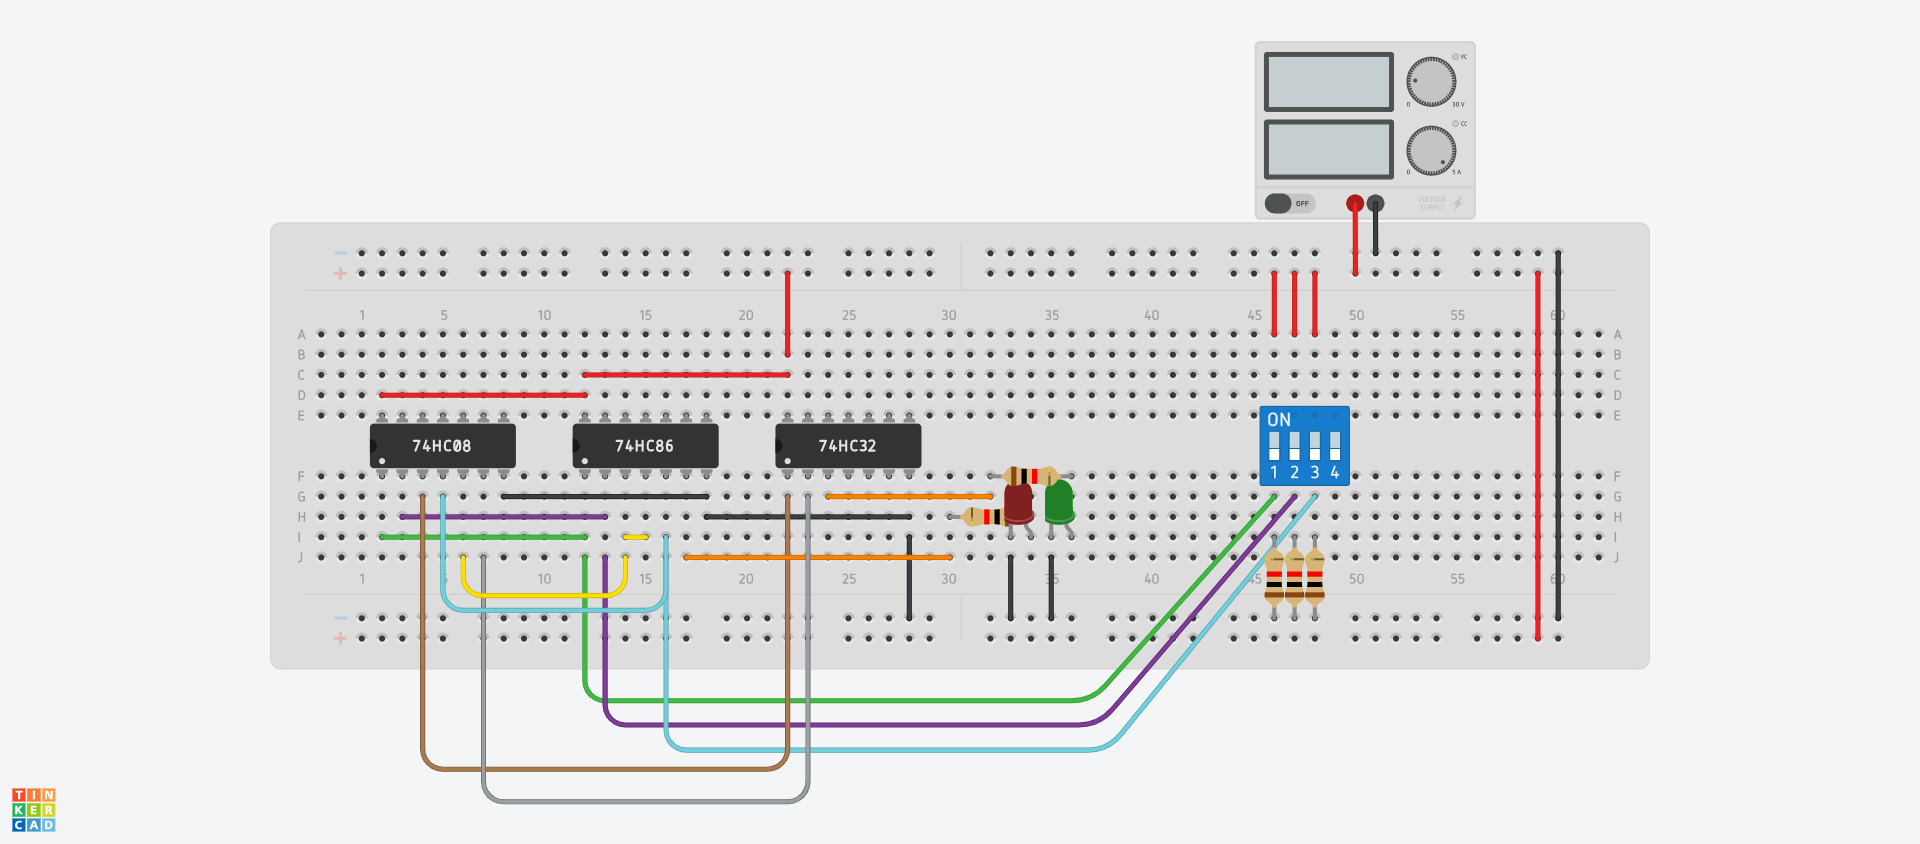
\includegraphics[width=1\textwidth, scale=2]{schematic.png}
  \caption*{My breadboard setup for this lab session.}
  \label{fig:schem}
\end{figure}
\vspace*{\fill}
\newpage
\topskip0pt
\vspace*{\fill}
\begin{center}
  {\Huge\textbf{\underline{All possible input combinations}}}
\end{center}
\vspace*{\fill}
\newpage
\begin{figure}
     \centering
     It is to be noted that the \textbf{red LED} stands for the $S$ bit (\textit{the sum bit}) and that the \textbf{green LED} stands for the $C_{out}$ bit (\textit{the carry bit}). A more intuitive view of binary addition through this 1-bit full adder could have been achieved by arranging the $C_{out}$ LED before the $S$ LED (\emph{opposite of what is portrayed in pictures hereunder}).\vspace{1em}
     \begin{subfigure}[b]{0.9\textwidth}
         \centering
        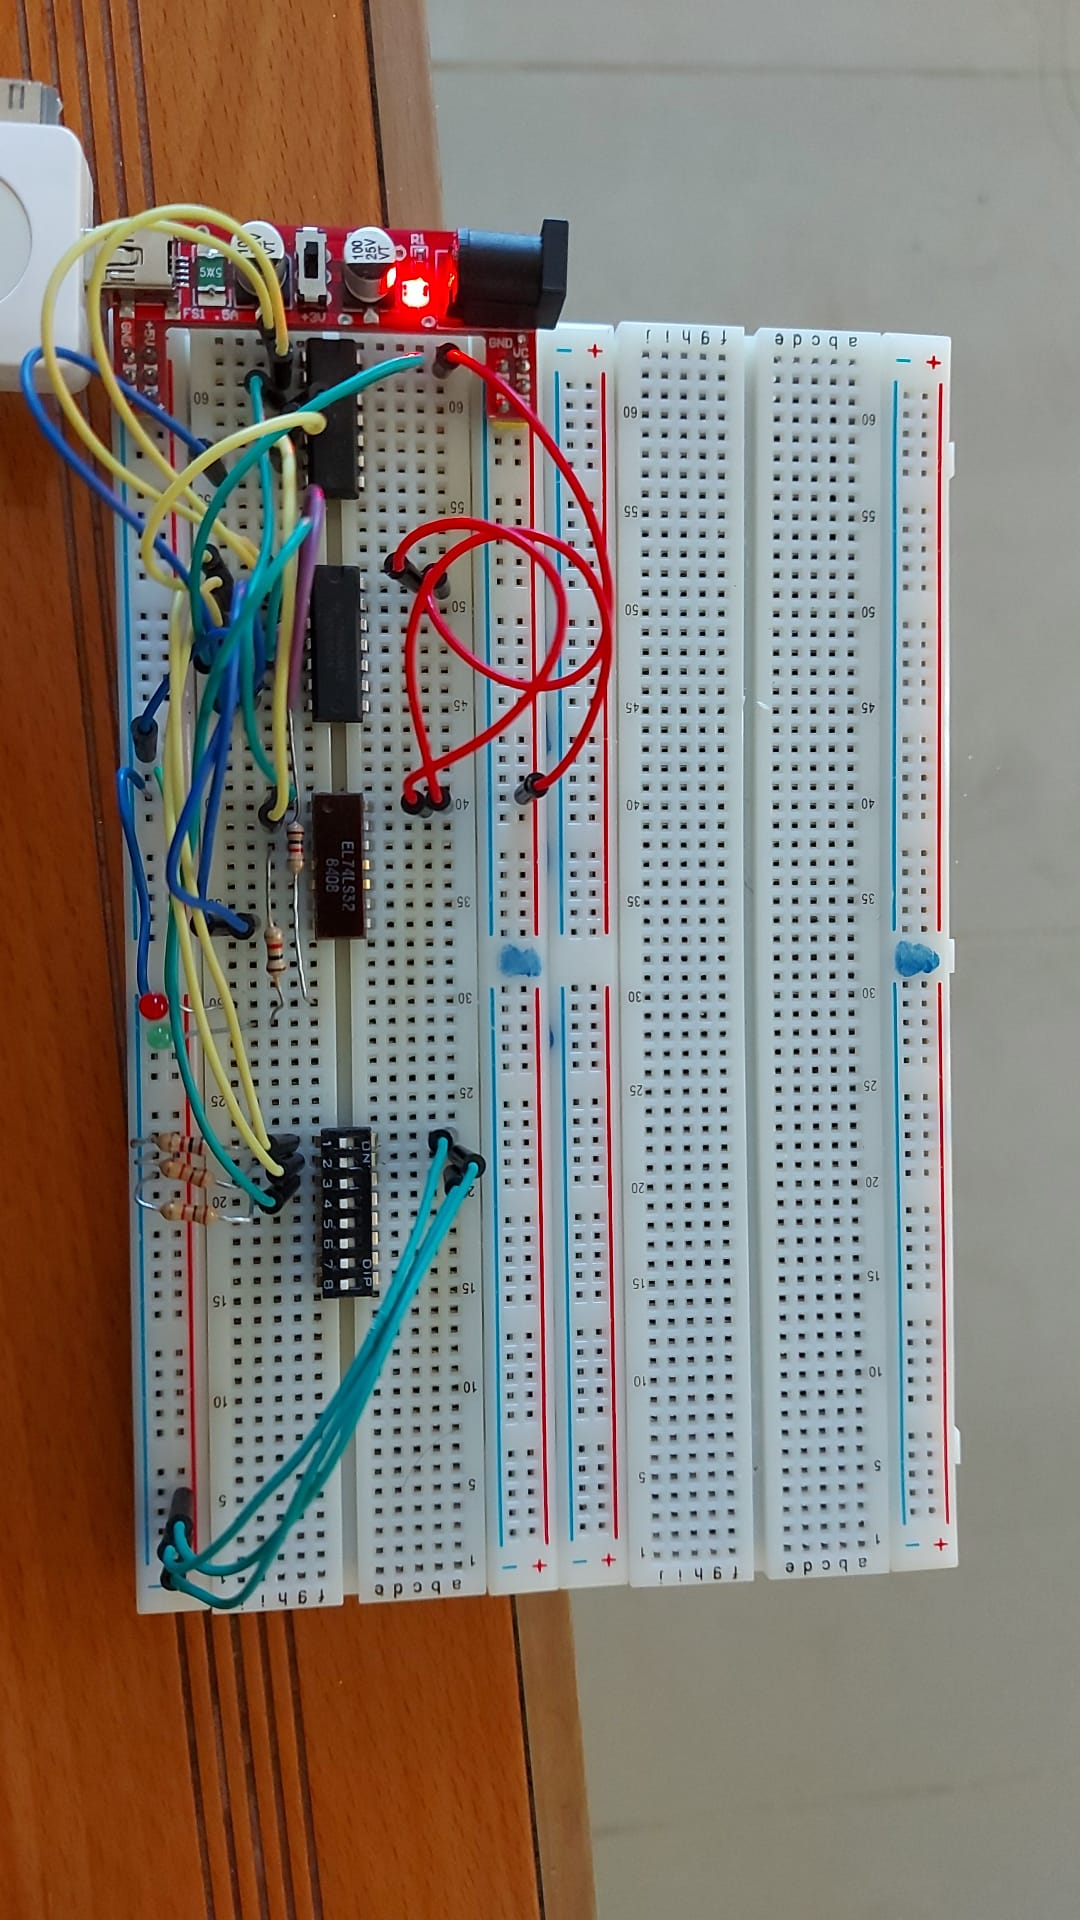
\includegraphics[angle=90, width=\textwidth]{alloff.jpeg}
        \caption*{\textbf{Figure 1.} All switches are off. $A=0,\,B=0,\, C_{in} = 0$ and so $S=0,\,C_{out}=0$.\vspace{2em}}
         \label{fig:alloff}
     \end{subfigure}
     \hfill
     \begin{subfigure}[b]{0.9\textwidth}
         \centering
         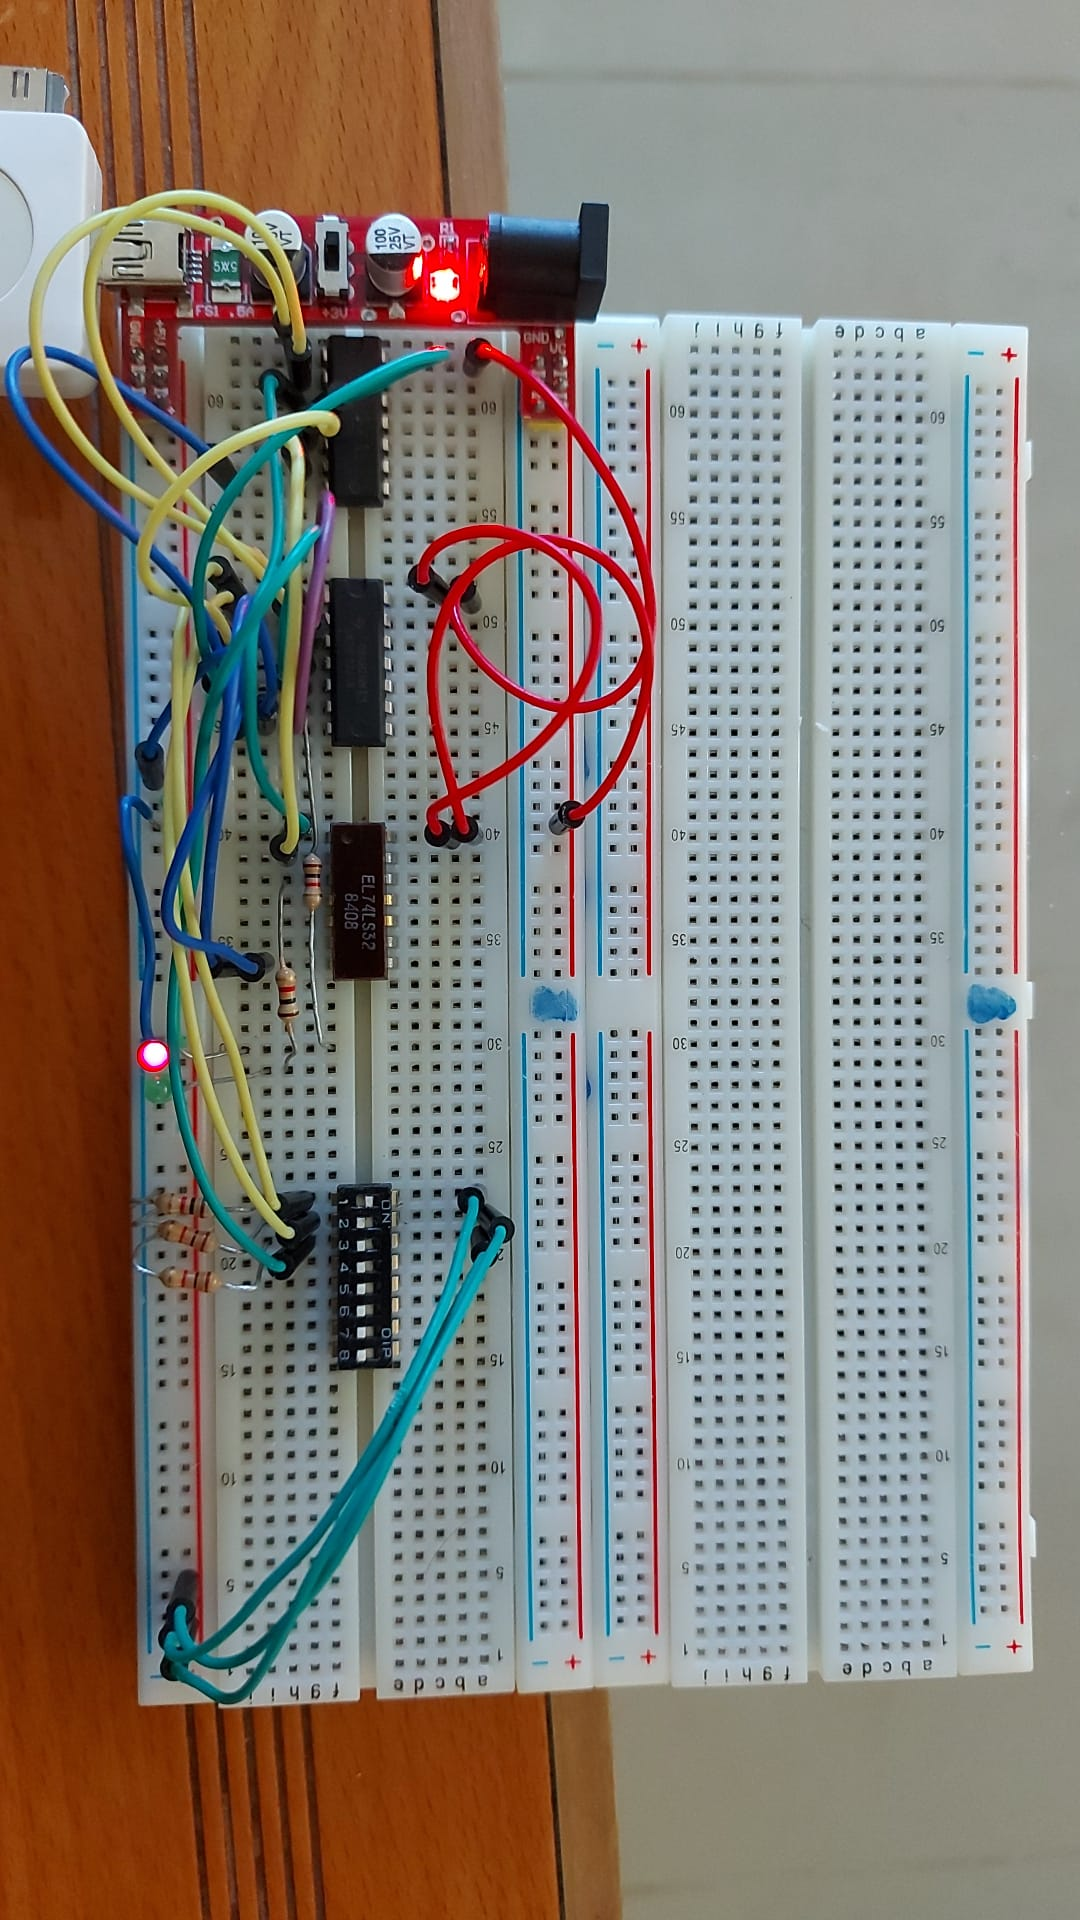
\includegraphics[angle=90, width=\textwidth]{1on.jpeg}
         \caption*{\textbf{Figure 2.} Only switch 1 is on. $A=1,\,B=0,\, C_{in} = 0$ and so $S=1,\,C_{out}=0$.\vspace{2em}}
         \label{fig:1on}
     \end{subfigure}
 \end{figure}
\newpage
\begin{figure}
     \centering
     \begin{subfigure}[b]{0.9\textwidth}
         \centering
          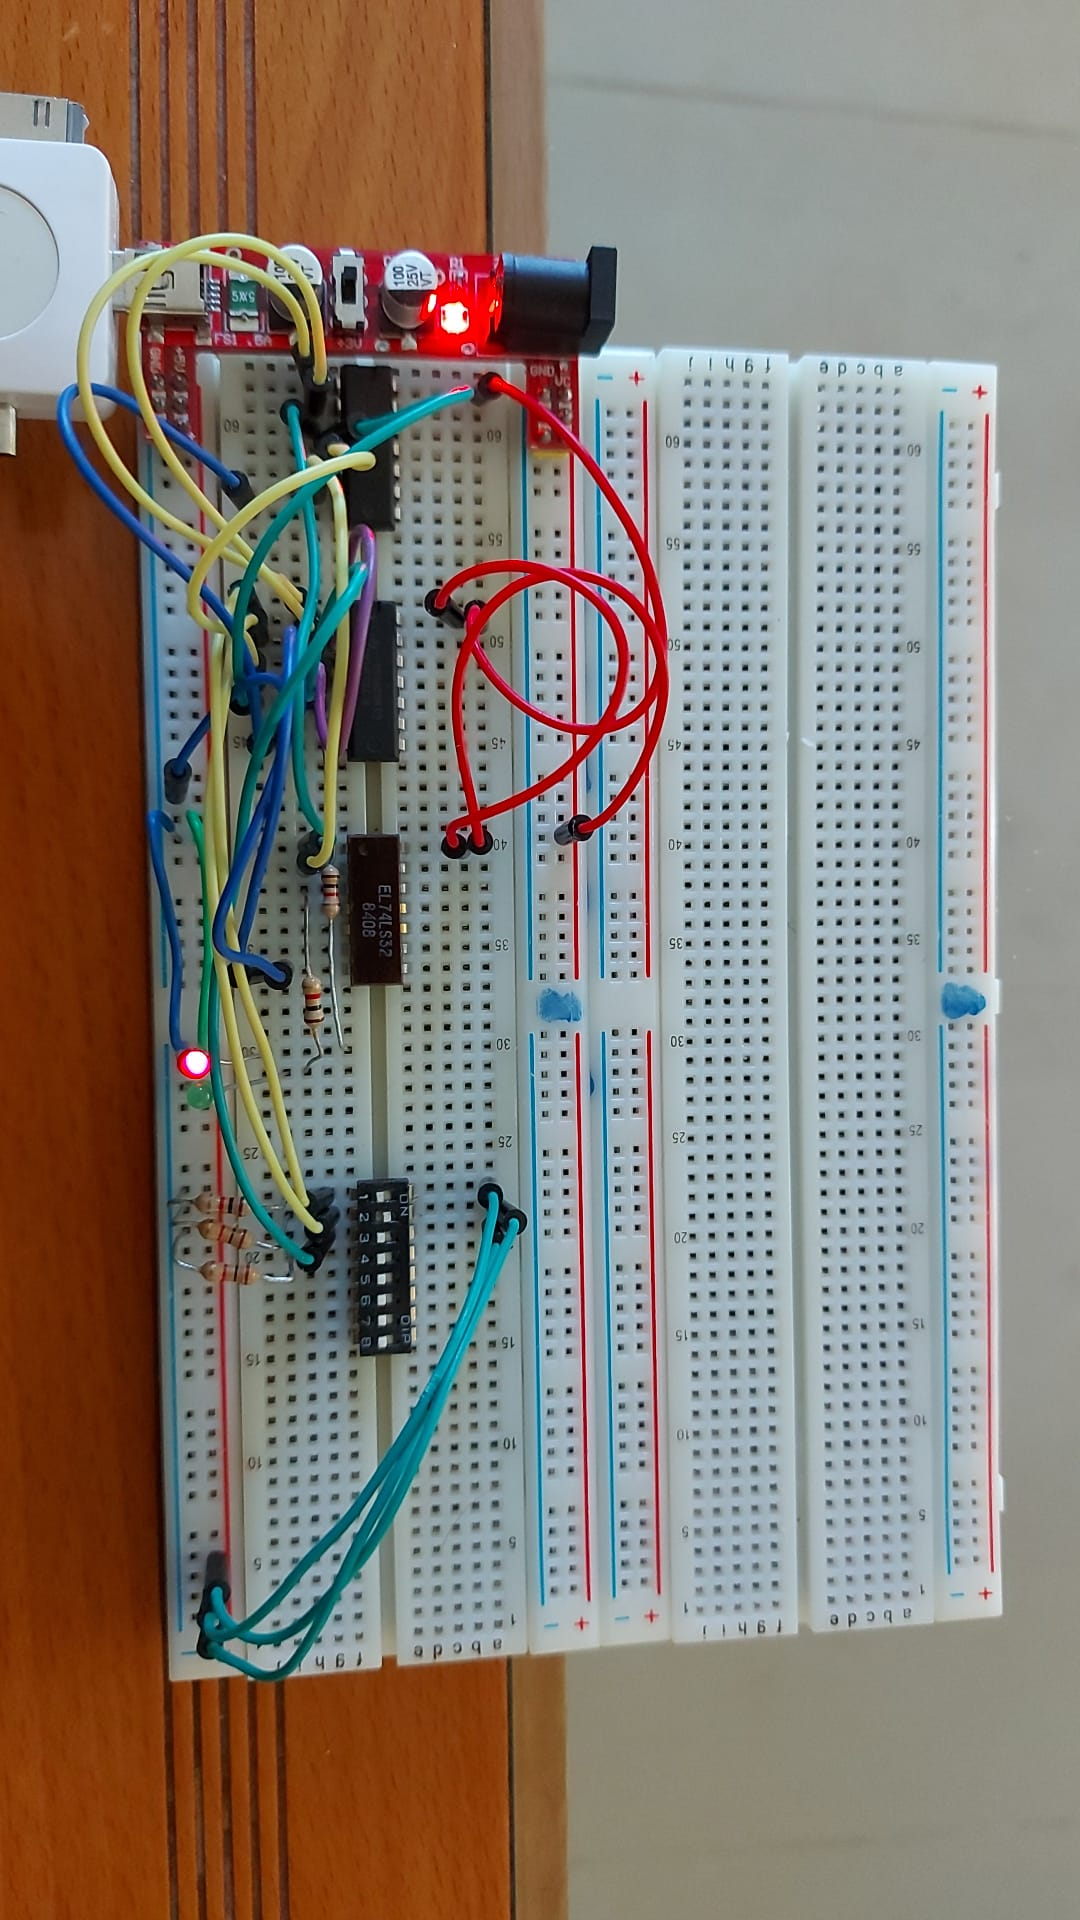
\includegraphics[angle=90, width=\textwidth]{2on.jpeg}
         \caption*{\textbf{Figure 3.} Only switch 2 is on. $A=0,\,B=1,\, C_{in} = 0$ and so $S=1,\,C_{out}=0$.\vspace{2em}}
         \label{fig:2on}
     \end{subfigure}
     \hfill
     \begin{subfigure}[b]{0.9\textwidth}
         \centering
        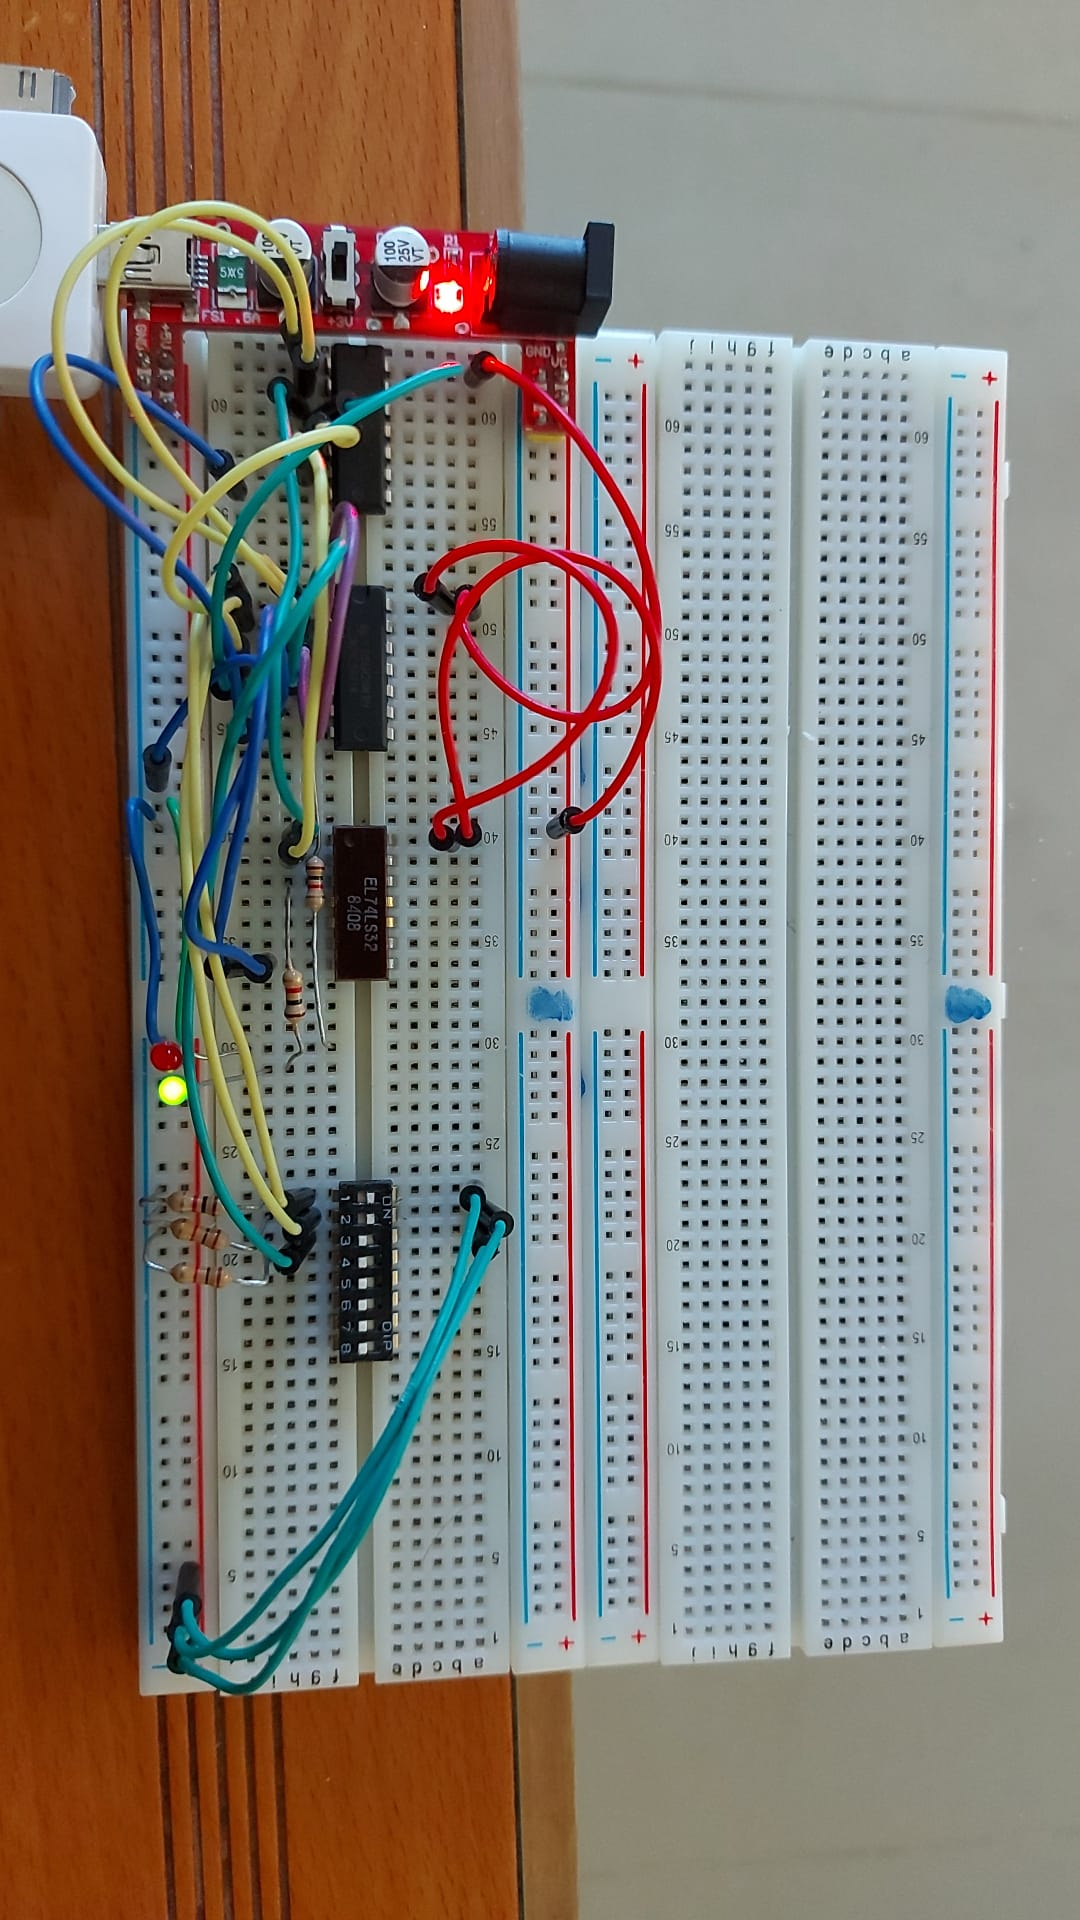
\includegraphics[angle=90, width=\textwidth]{12on.jpeg}
         \caption*{\textbf{Figure 4.} Only switches 1 and 2 are on. $A=1,\,B=1,\, C_{in} = 0$ and so $S=0,\,C_{out}=1$.\vspace{2em}}
         \label{fig:1on}
     \end{subfigure}
   \end{figure}
\begin{figure}
     \centering
     \begin{subfigure}[b]{0.9\textwidth}
         \centering
          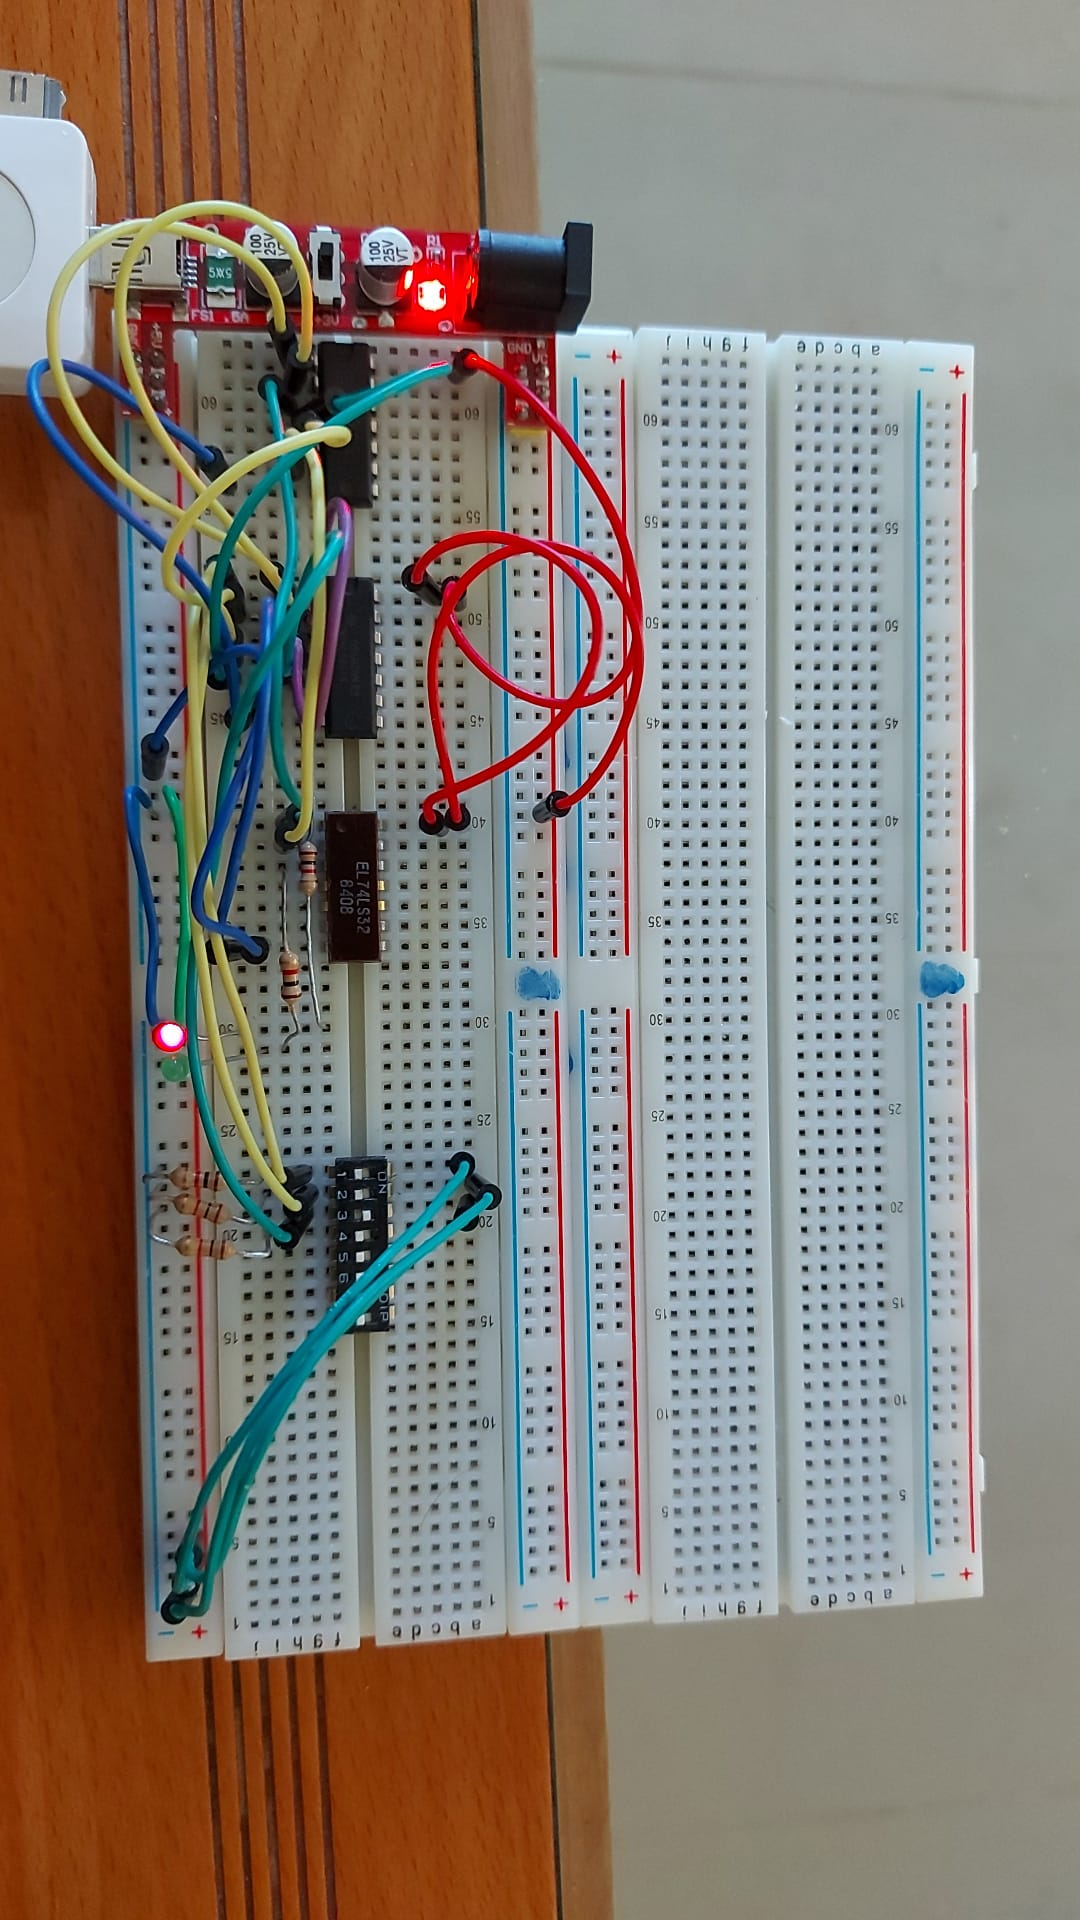
\includegraphics[angle=90, width=\textwidth]{3on.jpeg}
          \caption*{\textbf{Figure 5.} Only switch 3 is on. $A=0,\,B=0,\, C_{in} = 1$ and so $S=1,\,C_{out}=0$.\vspace{2em}}
         \label{fig:2on}
     \end{subfigure}
     \hfill
     \begin{subfigure}[b]{0.9\textwidth}
         \centering
        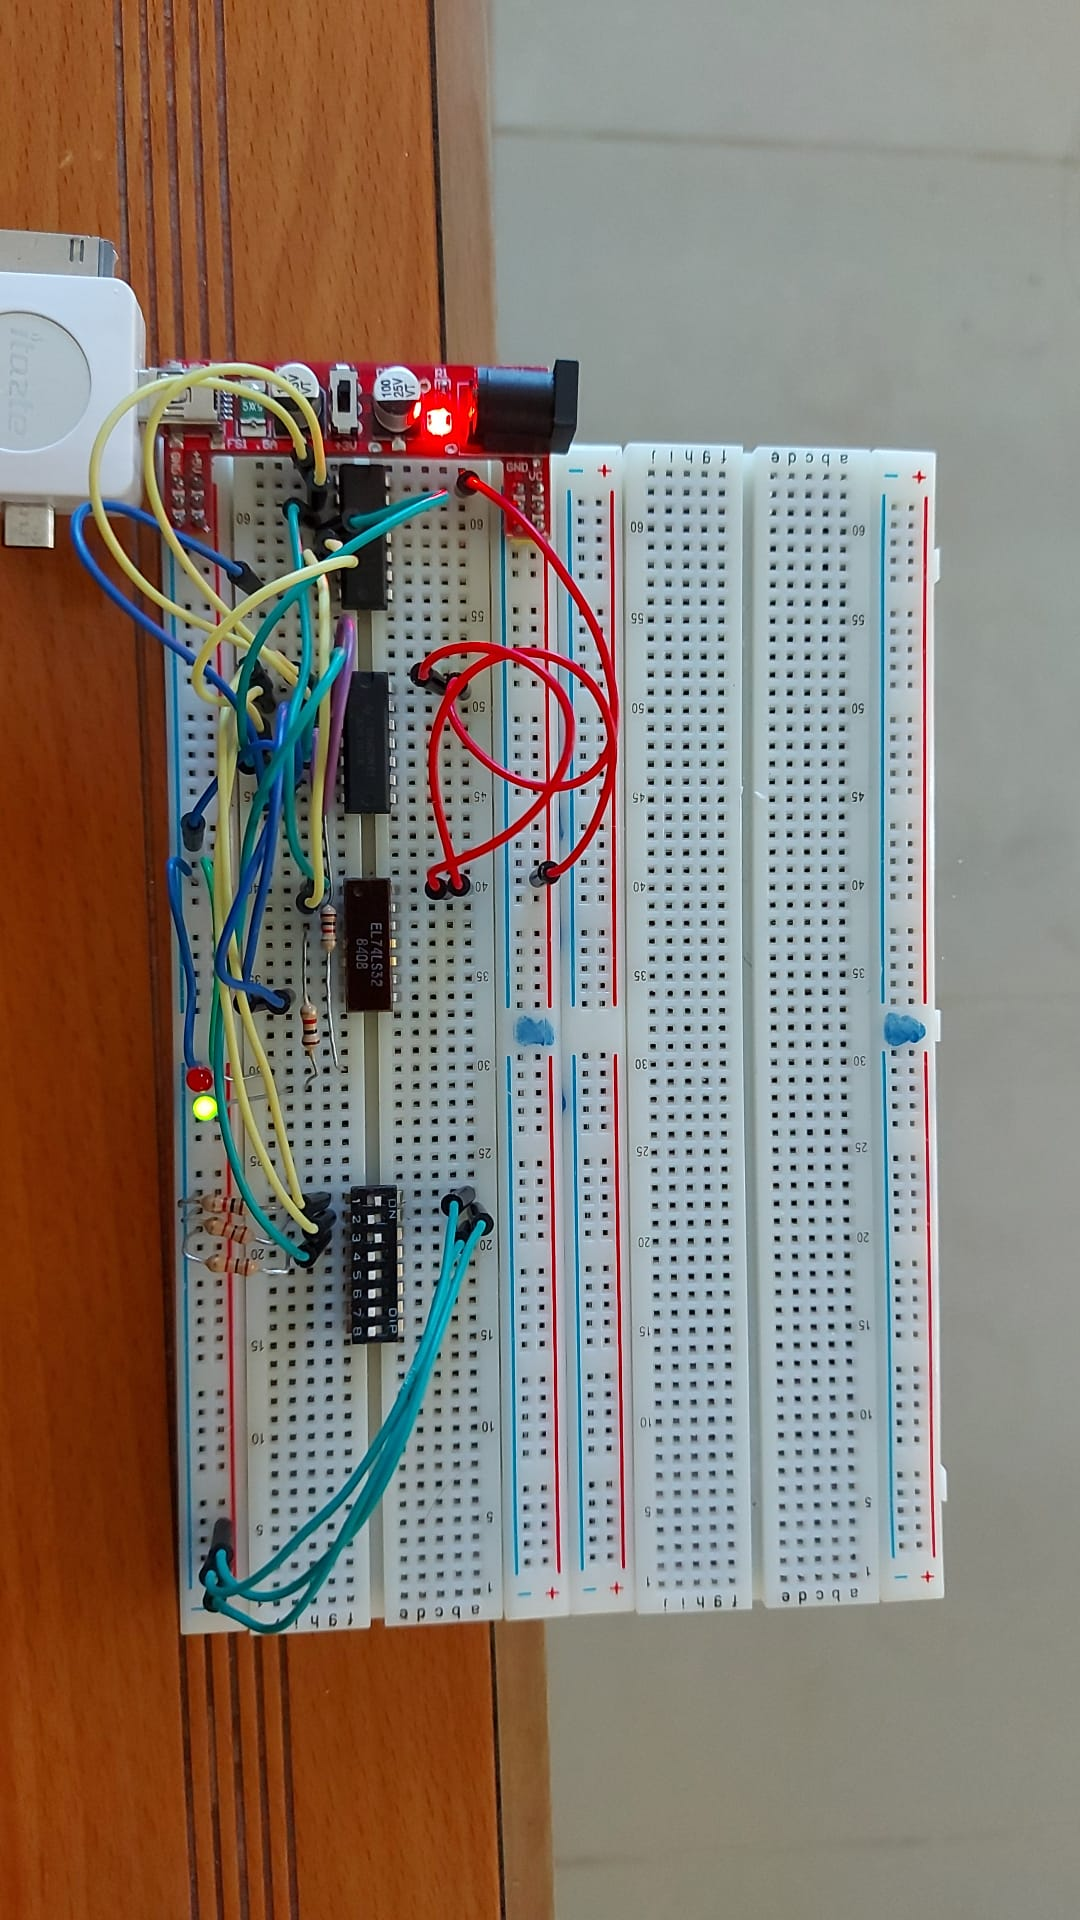
\includegraphics[angle=90, width=\textwidth]{13on.jpeg}
          \caption*{\textbf{Figure 6.} Only switch 1 and 3 are on. $A=1,\,B=0,\, C_{in} = 1$ and so $S=0,\,C_{out}=1$.\vspace{2em}}
         \label{fig:1on}
     \end{subfigure}
   \end{figure}
\begin{figure}
     \centering
     \begin{subfigure}[b]{0.9\textwidth}
         \centering
          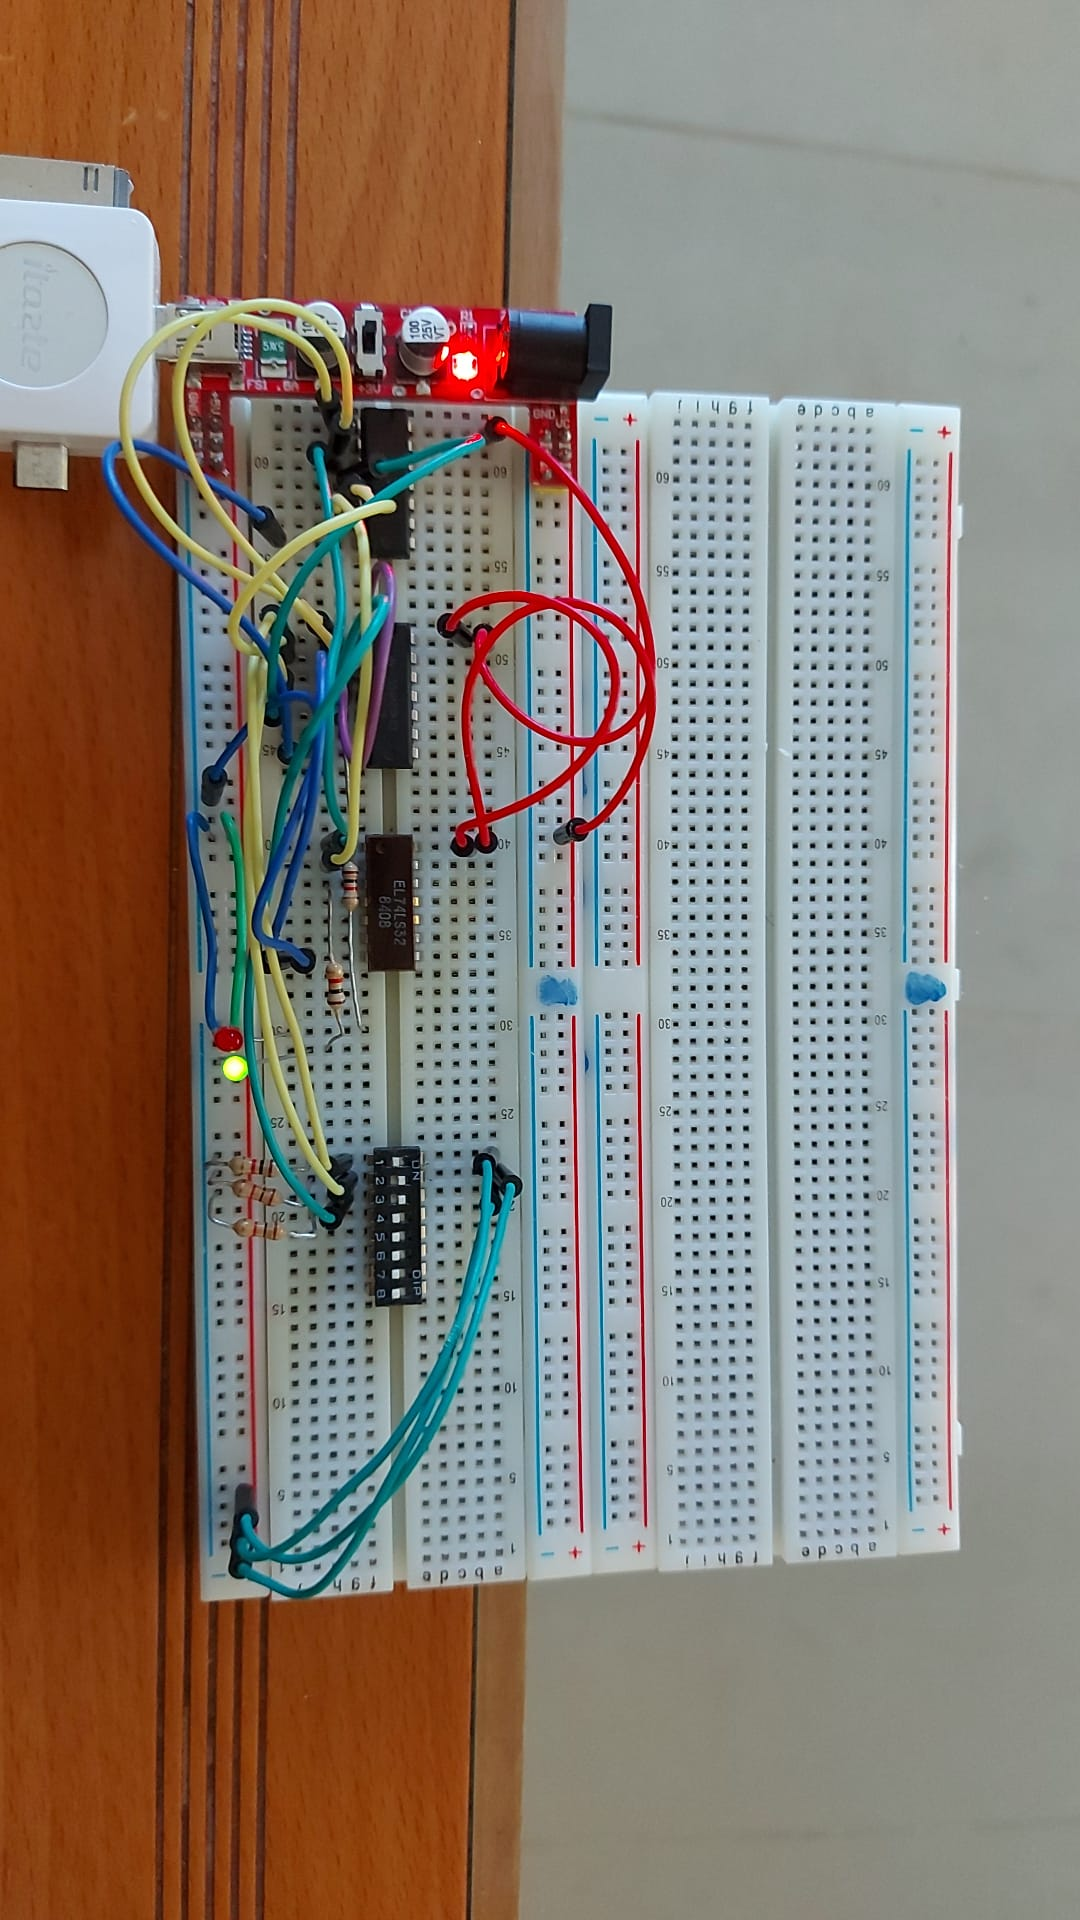
\includegraphics[angle=90, width=\textwidth]{23on.jpeg}
          \caption*{\textbf{Figure 7.} Only switches 2 and 3 are on. $A=0,\,B=1,\, C_{in} = 1$ and so $S=0,\,C_{out}=1$.\vspace{2em}}
         \label{fig:2on}
     \end{subfigure}
     \hfill
     \begin{subfigure}[b]{0.9\textwidth}
         \centering
        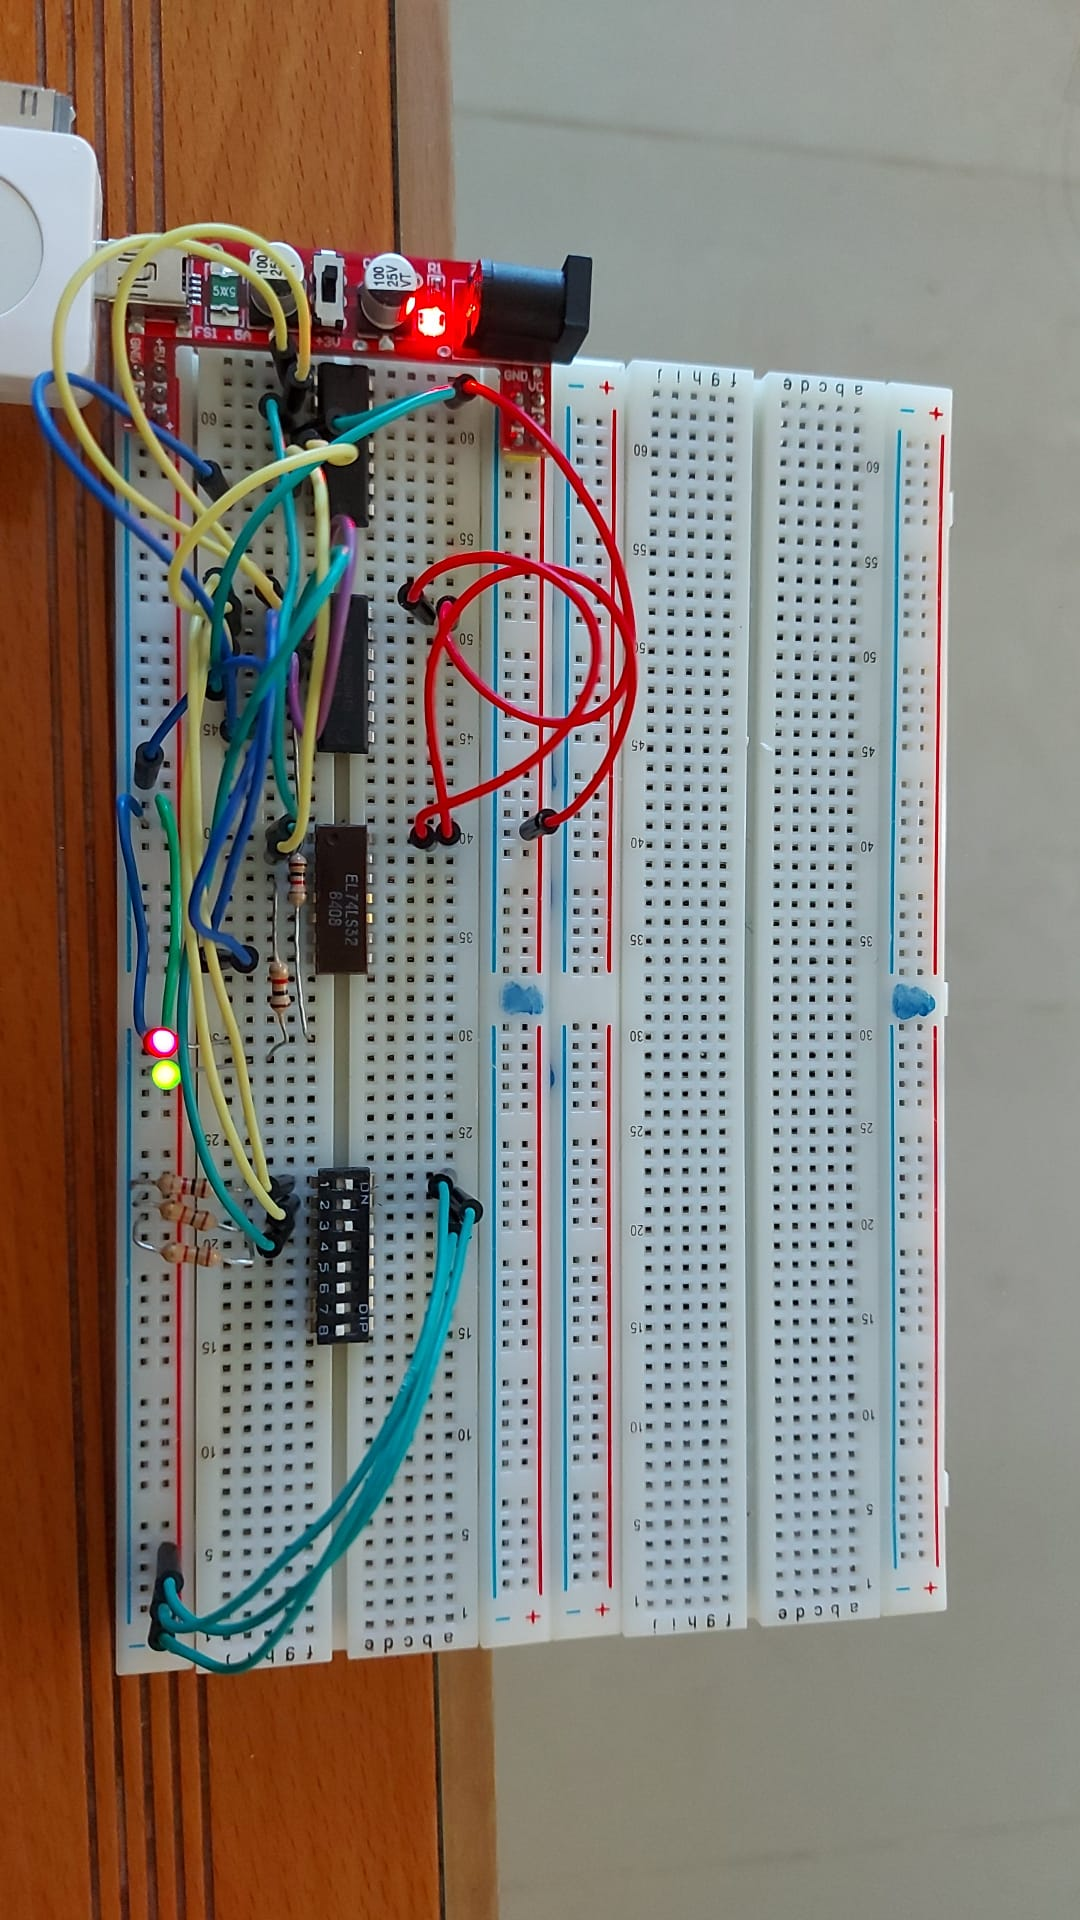
\includegraphics[angle=90, width=\textwidth]{123on.jpeg}
        \caption*{\textbf{Figure 8.} All switches are on. $A=1,\,B=1,\, C_{in} = 1$ and so $S=1,\,C_{out}=1$.\vspace{2em}}
         \label{fig:1on}
     \end{subfigure}
   \end{figure}
\end{document}
